
\section{Overview of the NIKA2 instrument}% {\color{YellowGreen} Nico}}

NIKA2 is a millimeter camera able to simultaneously image a field-of-view of
6.5\,arcmin in diameter at 150 and 260~GHz, with polarimetric capabilities at
260~GHz. The optics of the telescope receiver cabin have been modified in order
to increase the telescope field-of-view compared to earlier IRAM instruments. To
achieve these goals without degrading the telescope angular resolution, it
employs a total of around 2,900\,detectors split over three distinct arrays of
Kinetic Inductance Detectors (KID). A KID is a planar superconducting resonator
properly designed to absorb the incoming radiation and at the same time
incarnate the multiplexing scheme. The resonance quality factors of the KID used in NIKA2
are of the order of 15,000.
The measurable quantity, proportional to the
incoming power per pixel, is the shift in frequency of each resonance
(pixel). This shift is a consequence of variations of the resonator (kinetic)
inductance with incoming radiation.

\subsection{Optics}

The NIKA2 camera optics include two cold mirrors, and the filtering of unwanted
(off-band) radiation is provided by a suitable stack of multi-mesh filters
placed at all temperature stages between 150 mK and room temperature. An air-gap
dichroic splits the 150\,GHz (reflection) from the 260\,GHz (transmission)
beams. A grid polariser ensures then the separation of the two linear
polarizations on the 260\,GHz channel (V and H). Band-defining filters,
custom-designed to optimally match the atmospheric windows, are installed in
front of each array. A half-wave polarization modulator is added at room
temperature when operating the instrument in polarimetric mode.


%-------------------------
% HERVE



\subsection{Bandpasses {\color{blue} Herv\'e} }
\label{se:bandpasses}

\begin{figure}[ht!] % Inline image example
\begin{center}
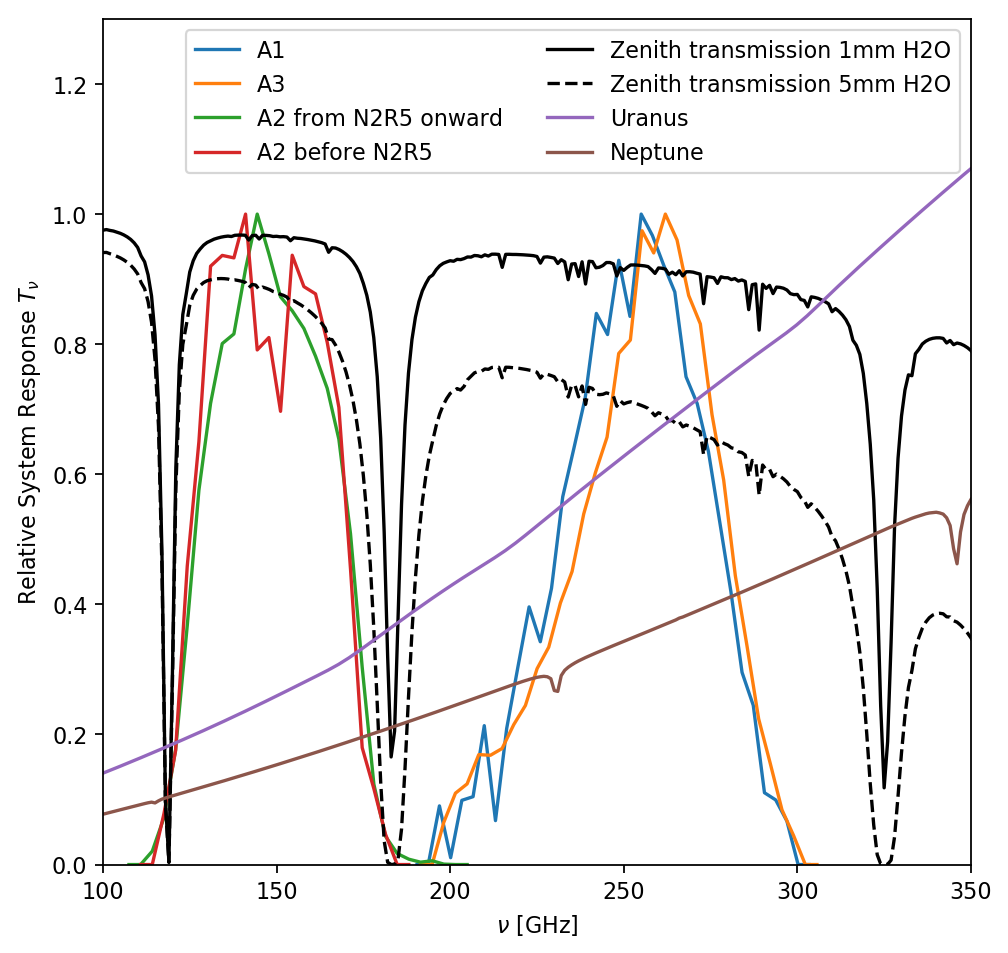
\includegraphics[width=0.75\textwidth]{Figures/SpectralBands/bandpasses_nika2.png}
\caption[NIKA2 transmission]{Relative system response of the three NIKA2 arrays as a
  function of frequency. For illustration we also plot atmospheric transmission obtained with the ATM model 
 \cite{ATM} for different values of precipitable water vapor. The spectra of ESA4 model of Uranus and ESA5 model of Neptune \cite{ESAmodel} in the frequency range are overplotted with arbitrary normalization.} 
 \label{spectralband1}
\end{center}
\end{figure}

 

The NIKA2 spectral bands were measured in the laboratory using a
Martin-Puplett interferometer built in-house \cite{durand}.  Both
arrays and filter bands were considered in the measurements. These
were obtained from the difference of two black bodies, hence they
include a $\nu^2$ Rayleigh-Jeans (RJ) spectral term.
Figure~\ref{spectralband1} shows the relative spectral response for
the three arrays (corrected of the RJ term).  Notice that array A2 was
replaced by a new one in N2R5 and that the spectral transmissions are
not the same (green and red lines in the figure).

The two arrays operating at 260 GHz, mapping different polarisations,
exhibit a slightly different spectral behaviour probably as can be
seen on figure \ref{spectralband1}. This may be explained by a tiny
difference in the silicon wafer and/or Aluminium film thicknesses. For
instance, the observed shift of the peak frequency, 265 GHz for the V
(A1) array versus 258 GHz for the H one (A3), can be explained by
about 5 microns change in the substrate thickness. Hereafter, the peak
frequencies are referred to as reference frequencies (150 and 260 GHz)
to which correspond the reference wavelengths (2.0 and 1.15 mm), see
tab.~\ref{tab:nika2summary}.


\begin{table}[th]
\begin{center}
\begin{tabular}{|l|l|r|r|r|r|r|r|}
\hline 
\multirow{3}{*}{Water vapor} & \multirow{3}{*}{Elevation} & \multicolumn{2}{|c|}{1 mm (H)} & \multicolumn{2}{|c|}{1 mm (V)} &
\multicolumn{2}{|c|}{2 mm} \\
 & & $\nu_eff$ & $\Delta \nu$  & $\nu_eff$ & $\Delta \nu$  & $\nu_eff$ & $\Delta \nu$ \\
 & & (GHz) & (GHz)  & (GHz)  & (GHz)   & (GHz)  & (GHz)  \\
\hline
\multicolumn{2}{|c|}{No atmosphere} & 254.71 & 49.21 & 257.39 & 48.05 & 150.93 & 40.72 \\
\hline
\multirow{4}{*}{1 mm $\rm H_2O$ $\rightarrow \tau_{225}=$0.067} & 90 deg &  254.46 & 48.72 & 257.12 & 47.95 & 150.93 & 39.71 \\
 & 60 deg & 254.42 & 48.68 & 257.08 & 47.93 & 150.92 & 39.60 \\
 & 40 deg & 254.33 & 48.57 & 256.98 & 47.89 & 150.88 & 39.32 \\
 & 20 deg & 254.00 & 48.21 & 256.62 & 47.77 & 150.75 & 38.45 \\
\hline
\multirow{4}{*}{2 mm $\rm H_2O$ $\rightarrow \tau_{225}=$0.120} & 90 deg &  254.26 & 48.74 & 256.91 & 48.06 & 150.64 & 39.34 \\
 & 60 deg & 254.20 & 48.70 & 256.84 & 48.07 & 150.60 & 39.19 \\
 & 40 deg & 254.02 & 48.60 & 256.65 & 48.08 & 150.48 & 38.80 \\
 & 20 deg & 253.43 & 48.30 & 256.01 & 47.93 & 150.13 & 37.62 \\
\hline
\multirow{4}{*}{3 mm $\rm H_2O$ $\rightarrow \tau_{225}=$0.173} & 90 deg &  254.06 & 48.76 & 256.70 & 48.19 & 150.39 & 39.03 \\
 & 60 deg & 253.97 & 48.73 & 256.60 & 48.21 & 150.32 & 38.84 \\
 & 40 deg & 253.71 & 48.65 & 256.33 & 48.28 & 150.14 & 38.35 \\
 & 20 deg & 252.86 & 48.41 & 255.40 & 47.86 & 149.60 & 36.94 \\
\hline
\multirow{4}{*}{5 mm $\rm H_2O$ $\rightarrow \tau_{225}=$0.278} & 90 deg &  253.67 & 48.82 & 256.28 & 48.45 & 149.96 & 38.47 \\
 & 60 deg & 253.51 & 48.81 & 256.11 & 48.44 & 149.84 & 38.22 \\
 & 40 deg & 253.10 & 48.77 & 255.68 & 48.26 & 149.54 & 37.58 \\
 & 20 deg & 251.74 & 48.67 & 254.20 & 47.75 & 148.68 & 35.82 \\
\hline
\multirow{4}{*}{8 mm $\rm H_2O$ $\rightarrow \tau_{225}=$0.437} & 90 deg &  253.08 & 48.94 & 255.66 & 48.42 & 149.38 & 37.76 \\
 & 60 deg & 252.84 & 48.93 & 255.39 & 48.35 & 149.20 & 37.42 \\
 & 40 deg & 252.21 & 48.94 & 254.71 & 48.16 & 148.77 & 36.64 \\
 & 20 deg & 250.12 & 49.38 & 252.43 & 47.91 & 147.52 & 34.57 \\
\hline
\multirow{4}{*}{10 mm $\rm H_2O$ $\rightarrow \tau_{225}=$0.542} & 90 deg &  252.70 & 49.00 & 255.24 & 48.38 & 149.04 & 37.34 \\
 & 60 deg & 252.39 & 49.01 & 254.92 & 48.29 & 148.82 & 36.97 \\
 & 40 deg & 251.62 & 49.11 & 254.08 & 48.13 & 148.31 & 36.12 \\
 & 20 deg & 249.07 & 49.75 & 251.28 & 48.24 & 146.85 & 33.93 \\
\hline
\end{tabular}
\caption[Effective frequencies and bandwidthes]{Effective frequencies (for Uranus) and bandwidth of the NIKA2 bands for
  various atmospheric conditions and elevation.}
\label{tab:bandwidths}
\end{center}
\end{table}

%What actually matters more than the ``central frequency'' that depends on many
%assumptions and definitions are the bandpasses. We should make available in a
%.fits file, clearly, our bandpasses to avoid future misunderstanding and propagation of
%false numbers. Official values should be 150 and 260~GHz. We should also clearly
%state that these measured bandpasses were done with the difference of two
%black-bodies, hence they include a $\nu^2$ RJ term.\\

{\color{red} LP: to be moved to Section Calibration ? Opacity ? }


The total system response is the multiplication of the atmospheric
transmission with the relative system response. To derive the
atmospheric transmission, we use GILDAS ATM 2009 model \cite{ATM}, computed for
the IRAM 30-m telescope, with so called {\it midlatwinter} conditions. We select in the model
grid an atmosphere with $T=268.3 \ {\rm K}$ and a pressure of $703.5 \ {\rm hPa}$. The
effective frequency of the passband is defined by:
\begin{equation}
\nu_{eff}( \sec \delta, mm_{H_{2}O}) = \frac{ \int_{0}^{+\infty} S_{\nu}
  T_{\nu}(\sec \delta, mm_{H_{2}O}) \nu d\nu } { \int_{0}^{+\infty} S_{\nu} T_{\nu} d\nu}
\label{eq:nueff0}
\end{equation}

{\color{blue} FXD: we should integrate over SOmega (nu-2). For
  MartinPuplett measurements, the source spectrum was RJ (nu2) so that
  cancels out to find Tnu. Snu is for an extended source. Deltanu
  should be with respect to a spectrum, for example RJ. I think the
  table 2.1 is not very useful. It could be a figure (nueff as a
  function of tauLOS (elevation is not relevant)? or just few numbers:
  we should at the end state what is nueff and deltanu for average
  conditions. Nomenclature: 1mm(H) is not the usual denomination... }


where $T_{\nu}$ is the total system response, normalized between
0. and 1. (i.e. a relative response as a function of the frequency),
hereafter referred to as RSR (Relative System Response), $S_{\nu}$ is
the source spectrum. Table~\ref{tab:bandwidths} lists this effective frequency,
computed for Uranus spectrum (ESA4 model, \cite{ESAmodel}), for different atmospheric
water vapor contents and different elevations. 
Table~\ref{tab:bandwidths} also list the bandwidth, defined as:
\begin{equation}
\Delta\nu = \int_{0}^{+\infty} \frac{T_{\nu}}{Max(T_{\nu})}
d\nu
\end{equation}
where the $Max(T_{\nu})$ ensure the RSR span the whole 0.0 to 1.0 range.

From Table~\ref{tab:bandwidths}, we see that the 2 mm band is somewhat
sensitive to the atmospheric conditions, especially at low
elevation. Note that these effective frequencies are {\em not} the
reference frequencies for the band, respectively 150 GHz and 260 GHz
for the A2 and A1, A3 arrays. These reference frequencies are chosen
as round numbers in the middle of the bands to define NIKA2
photometric system as will be discussed in section~\ref{se:cal_HA}.

%
% LP: the paragraph below rather belongs to the Opacity section
%
%Using the NIKA2 bandpasses for N2R9, we can integrate the ATM
%atmospheric model to compute the expected ratio between the
%atmospheric opacity of the two NIKA2 channels. 
%Figure~\ref{thopacities} shows the atmospheric opacity
%ratio of the 2 and 1 mm channels as a function of the opacity for the
%1 mm one.

%\begin{figure}[ht] % Inline image example
%\begin{center}
%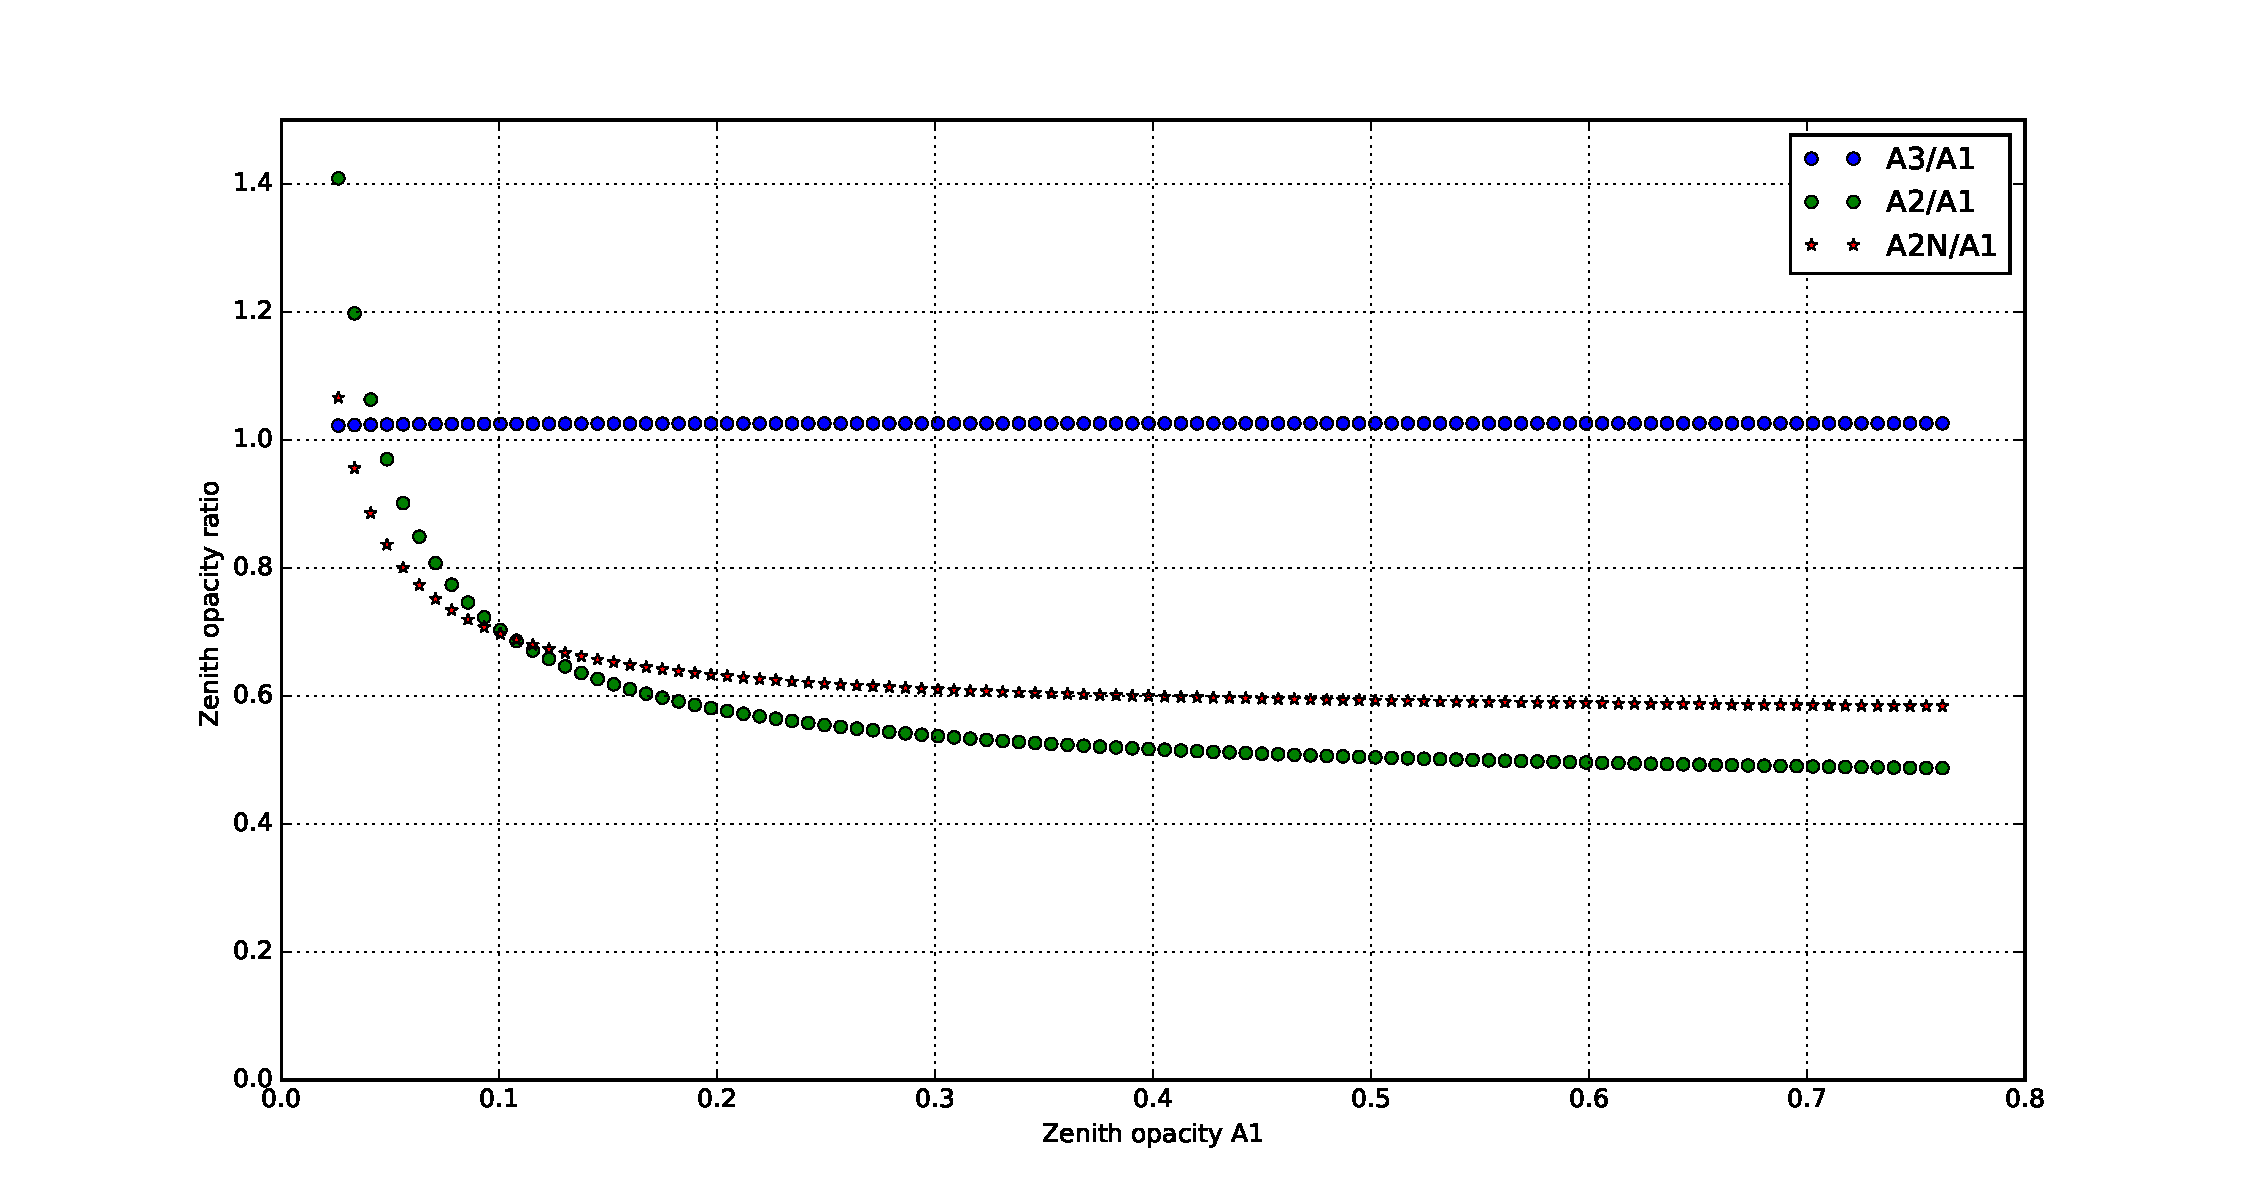
\includegraphics[width=\textwidth]{Figures/SpectralBands/opacity_ratio_vs_tau1.pdf}
%\caption{Expected atmospheric opacity ratio of the 2 and 1 mm channels as function 
%of the opacity at 1 mm. {\bf FM: what is A2N/A1 ?} {\bf FM: why is A3/A1=1 ?}}
%\label{thopacities}
%\end{center}
%\end{figure}





%-------------------------

\subsection{Cryogenics}

The optimal operation of the detectors is achieved at a temperature of around
150\,mK, well below the Aluminium superconducting transition. For this reason,
NIKA2 employs a custom dilution fridge to cool down the focal plane, and the
refractive portion of the optics, for a total mass around 100 kg, deeply in the
sub-Kelvin regime. Despite the complexity and size of the system, the operation
of NIKA2 does not require external cryogenic liquids and is fully remotely
controllable.

\subsection{KIDs and electronics}
\label{se:array}

The 150\,GHz channel is equipped with A2 that is an array of
616\,pixels, arranged to cover a 78\,mm diameter circle. Each pixel has a size of
$2.8\times2.8\textrm{\,mm}^2$. The array A2 is connected over four different
readout lines. In the case of the 260\,GHz band detectors, the pixel size is
$2\times 2\mathrm{\,mm}^2$, to ensure a comparable sampling of the focal
plane. In order to fill the two 260\,GHz arrays A1 and A3, a total of 1,140 pixels are
needed in each of them. The focal planes are all based on thin Aluminium films
deposited by e-beam evaporation under ultra-high vacuum conditions over a
Silicon substrate.

The key advantage of the KID technology is the simplicity of the cold
electronics and the multiplexing scheme. In NIKA2, each block of around 150
detectors is connected to single coaxial line providing the excitation and the
readout at the two ends. Each of the readout lines is linked to the input of a
cryogenic (4 K) low-noise amplifier. The warm electronics required to digitize
and process the pixels signals is composed of twenty custom readout cards (one
per feed-line).

%In this document, the 2\,mm array is called A2, while the two 1\,mm arrays are
%called A1 and A3.


\subsection{KID photometry and tuning}
\label{se:tuning}

\begin{figure}[!b]
\begin{center}
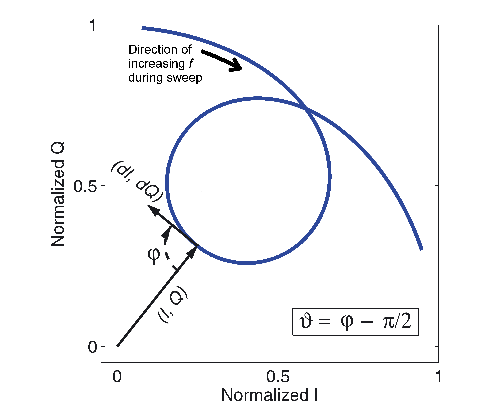
\includegraphics[width = 0.7\textwidth]{Figures/resoCircle-eps-converted-to.pdf}
\caption[KID resonance circle]{Sample resonance circle in the IQ plane. Both the
  tuning procedures are based on the measurement of the angle $\vartheta$
  between the two vectors ($I, Q$) and ($dI, dQ$)}
\label{figResoCircle}
\end{center}
\end{figure}

Kinetic Inductance Detectors are superconducting resonators whose resonance
frequency shifts linearly depend on the incoming optical power. The
measure of such frequency shift $\Delta f$ is what allows us to use
KID as mm-wave detectors.

For the KID readout, an excitation signal is sent into the cryostat on the
feedline coupled to the KID. The transmitted signal can be described by its
amplitude and phase, or, as is common practice for KID, by its components that
are In-phase ($I$) and in Quadrature $Q$ with respect to the excitation
signal. When a frequency sweep is carried around a KID resonance, the
transmitted signal makes a sort of circle in the $I-Q$ plane, as shown
in Fig.~\ref{figResoCircle}.
The goal is now to relate \sam{the measured variations of the KID response
to excitation signal} $(\Delta I, \Delta Q)$, which are induced by incident light, to
$\Delta f$. For this, the electronics modulates the excitation
frequency at about 1\,kHz with a known frequency variation $\delta f$
and the read out gives the induced transmitted signal variations
$(dI, dQ)$. Projecting linearly
$(\Delta I, \Delta Q)$ on $(dI, dQ)$ therefore
provides $\Delta f$. This value, in Hz, constitutes the raw
time-ordered data, which are sampled at a frequency of 23.84
Hz. Ingested into the calibration pipeline, it will be futher calibrated into astronomical units
(Sect.~\ref{se:calibration}). For historical reasons, this way of deriving KID
signals has been nicknamed \emph{RfdIdQ}. More details on this process are given
in \cite{Calvo13}.\\

Not only incident astronomical light reaches the KIDs and contributes to Cooper
pair breaking. Any change in the background optical load (due, for example, to changes in
the atmospheric transmission or in the elevation) contributes as well to the
shift of the resonances. In order to maximize the sensitivity of a KID, the
excitation signal used to read it out must always be near its resonance
frequency. We therefore have developped a tuning algorithm that takes care of
this optimization. Tunings are performed during the first subscan of each
observation in order to be optimally tuned at the same elevation and sky
conditions as the source. It takes only a few seconds when the $\ftone$ are
close to the current functionning point. In order to always be in these
conditions, continuous tunings are done between two scans when NIKA2 is not observing.

A specific case is when we do {\tt skydip} scans (see
Sect.~\ref{se:skydip}). In this case, we tune all the KIDs
at the beginning of each subscan, which corresponds to an elevation
step, on purpose to monitor the induced variation of $\ftone$ by the
sky load.

